% -*- coding: utf-8 -*-
%%%%%%%%%%%%%%%%%%%%%%%%%%%%%%%%%%%%%%%%%%%%%%%%%%%%%%%%%%%%%%%%%%%%%%%%%%%%%%%%
%2345678901234567890123456789012345678901234567890123456789012345678901234567890
%        1         2         3         4         5         6         7         8

%\UseRawInputEncoding


\documentclass[letterpaper, 10 pt, conference]{ieeeconf}  % Comment this line out if you need a4paper

%\pdfminorversion=4              % tell pdflatex to generate PDF in version 1.4
\usepackage[T1]{fontenc}
\usepackage{cite}
\usepackage{amssymb,amsfonts}
\usepackage{algorithmic}
\usepackage{graphicx}
\usepackage{textcomp}
\usepackage{changes}
\usepackage{subcaption}
\usepackage{xcolor}
\usepackage{color, soul}
\usepackage{amsmath}
\usepackage{booktabs}
\usepackage{multirow}
\usepackage{xstring}
%\documentclass[a4paper, 10pt, conference]{ieeeconf}      % Use this line for a4 paper

\IEEEoverridecommandlockouts                              % This command is only needed if 
                                                          % you want to use the \thanks command

\overrideIEEEmargins                                      % Needed to meet printer requirements.

%In case you encounter the following error:
%Error 1010 The PDF file may be corrupt (unable to open PDF file) OR
%Error 1000 An error occurred while parsing a contents stream. Unable to analyze the PDF file.
%This is a known problem with pdfLaTeX conversion filter. The file cannot be opened with acrobat reader
%Please use one of the alternatives below to circumvent this error by uncommenting one or the other
%\pdfobjcompresslevel=0
%\pdfminorversion=4

% See the \addtolength command later in the file to balance the column lengths
% on the last page of the document

% The following packages can be found on http:\\www.ctan.org
%\usepackage{graphics} % for pdf, bitmapped graphics files
%\usepackage{epsfig} % for postscript graphics files
%\usepackage{mathptmx} % assumes new font selection scheme installed
%\usepackage{times} % assumes new font selection scheme installed
%\usepackage{amsmath} % assumes amsmath package installed
%\usepackage{amssymb}  % assumes amsmath package installed
\usepackage{cite}

\title{\LARGE \bf
RONet: Real-time Range-only Indoor Localization via Stacked Bidirectional LSTM with Residual Attention}


\author{Hyungtae Lim$^{1}$ , Changgyu Park$^{2}$, Hyun Myung$^{3}$, \textit{Senior Member, IEEE}% <-this % stops a space
\thanks{
	*This material is based upon work supported by the Ministry of Trade, Industry \& Energy(MOTIE, Korea) under Industrial Technology Innovation Program. No.10067202, 'Development of Disaster Response Robot System for Lifesaving and Supporting Fire Fighters at Complex Disaster Environment'.}% <-this % stops a space
\thanks{$^{1}$Hyungtae Lim, $^{2}$Changgyu Park, and $^{3}$Hyun Myung are with
	the Urban Robotics Laboratory, Korea Advanced Institute of Science
	and Technology (KAIST) Daejeon, 34141, South Korea. {\tt\small shapelim@kaist.ac.kr, cpark@kaist.ac.kr, hmyung@kaist.ac.kr}}%
%
}


\begin{document}

\captionsetup[figure]{labelformat={default},labelsep=period,name={Fig.}}


\maketitle
\thispagestyle{empty}
\pagestyle{empty}


%%%%%%%%%%%%%%%%%%%%%%%%%%%%%%%%%%%%%%%%%%%%%%%%%%%%%%%%%%%%%%%%%%%%%%%%%%%%%%%%
\begin{abstract}


In this paper, a three-layered Bidirectional Long Short-Term Memory(Bi-LSTM) with residual attention, called RONet, is proposed. We gathered our own dataset and tested RONet in the real-world. Our RONet shows that it could estimate a position of the mobile robot in real-time, almost 32Hz on Nvidia Jetson AGX Xavier, using range-only observations.
 
 We also analyze sequence length of LSTM as a kind of hyper-parameters. We find that 8 sequence length is optimal among 2,3,5,8, and 12 sequence lengths in the way that building the network with 8 sequence length consider both covering uncertainty with more temporal information and estimating position precisely.

As verified experimentally, our RONet shows better precise performance  and robustness against outliers compared to a conventional range-only approach based on Particle Filter and deep learning-based approaches. We set three cases, reducing the number of anchors and check that our RONet is not only robust but also shows the least RMSE, 4.466cm, 3.210cm, 3.090cm in order of 3 anchors, 5 anchors, and 8 anchors are implemented respectively.   

\end{abstract}


%%%%%%%%%%%%%%%%%%%%%%%%%%%%%%%%%%%%%%%%%%%%%%%%%%%%%%%%%%%%%%%%%%%%%%%%%%%%%%%%
\section{INTRODUCTION}

In recent years, as demand for localization in indoor environments where the signals of Global Positioning Systems(GPS) could become imprecise gradually increases, many researchers have conducted various methods for locating objects, e.g., using magnetic fields, acoustic signals, or laser-based data. Among them, Time of Flight(TOF)-based range beacon sensors are widely utilized by virtue of characteristics of beacon sensors: low-cost, small-size, accurate performance, and convenience of being installed. As a result, these range measurement-based approaches have been suggested as a solution for localization  not only on the indoor environment\cite{peneda2009trilateration, jung2011indoor}, but also underwater environments\cite{newman2003pure, olson2006robust}
 
Specifically, these range-only approaches has addressed the problem of localization with sets of range-only measurements between a object node that we want to localize, called tag node, and landmarks, called anchor nodes. However, range measurements that only represent distances between each landmark and the mobile robot respectively. In other words, a set of one-dimensional data have two problems: one is that range-only observations tend to be non-linear because TOF-based measurement is very vulnerable to noise and has huge uncertainties caused by the multipath fading channel(MPF) problem\cite{li2017novel} in the real-world, and the other one is that these range-only observations have \textit{rank deficiency} problem\cite{fabresse2018efficient}. To be specific, the single value to represent the distance between each landmark and the mobile robot respectively is deficient to describe the exact position or orientation of the landmark so cause multimodal distribution\cite{gonzalez2009mobile}. 

\begin{figure}[h]
	
	\centering
	%\subfigure[]{
	%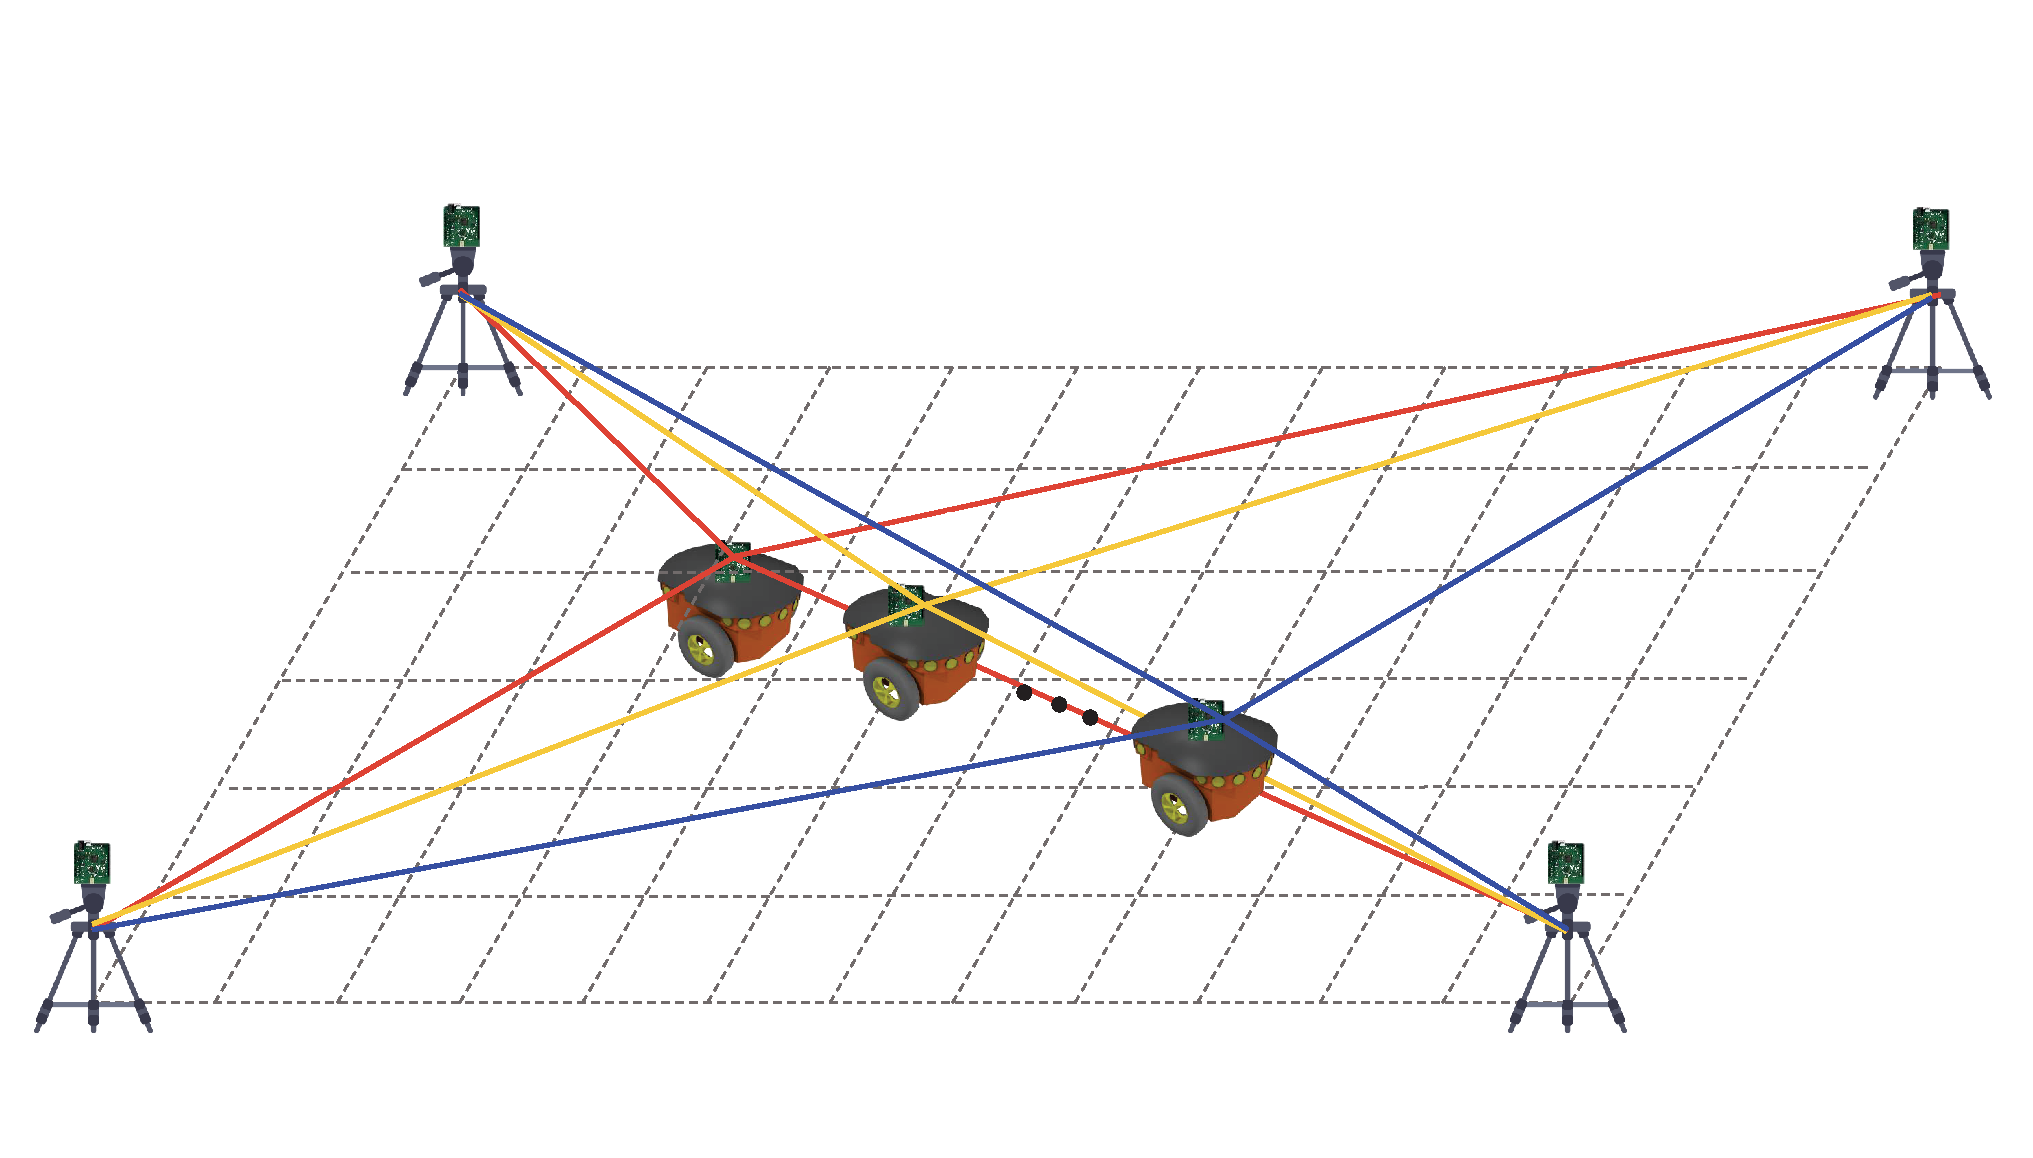
\includegraphics[height=4.5cm]{IROS2018_image_1}
	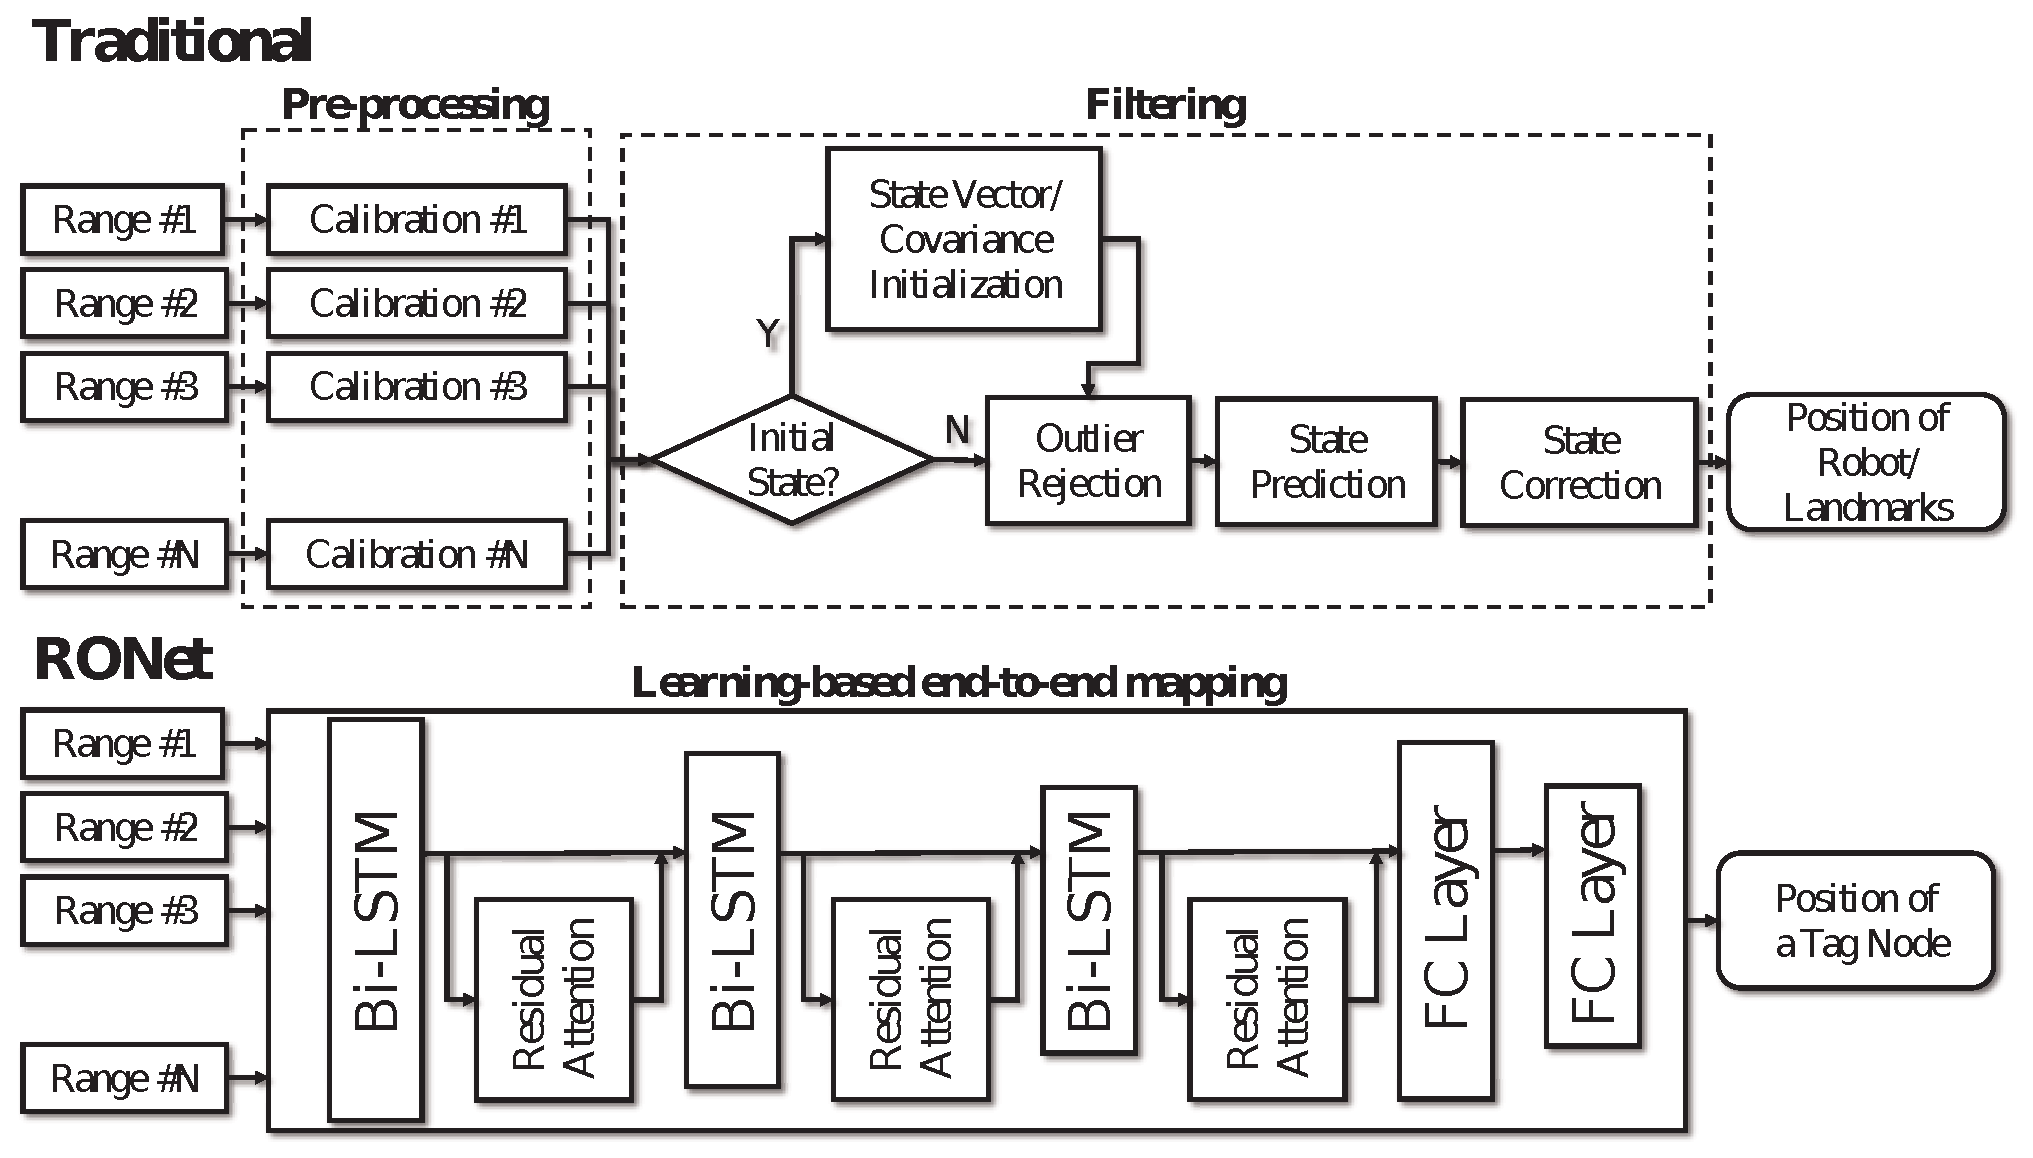
\includegraphics[height=5cm]{image/conventional_deep_v2}
	
	%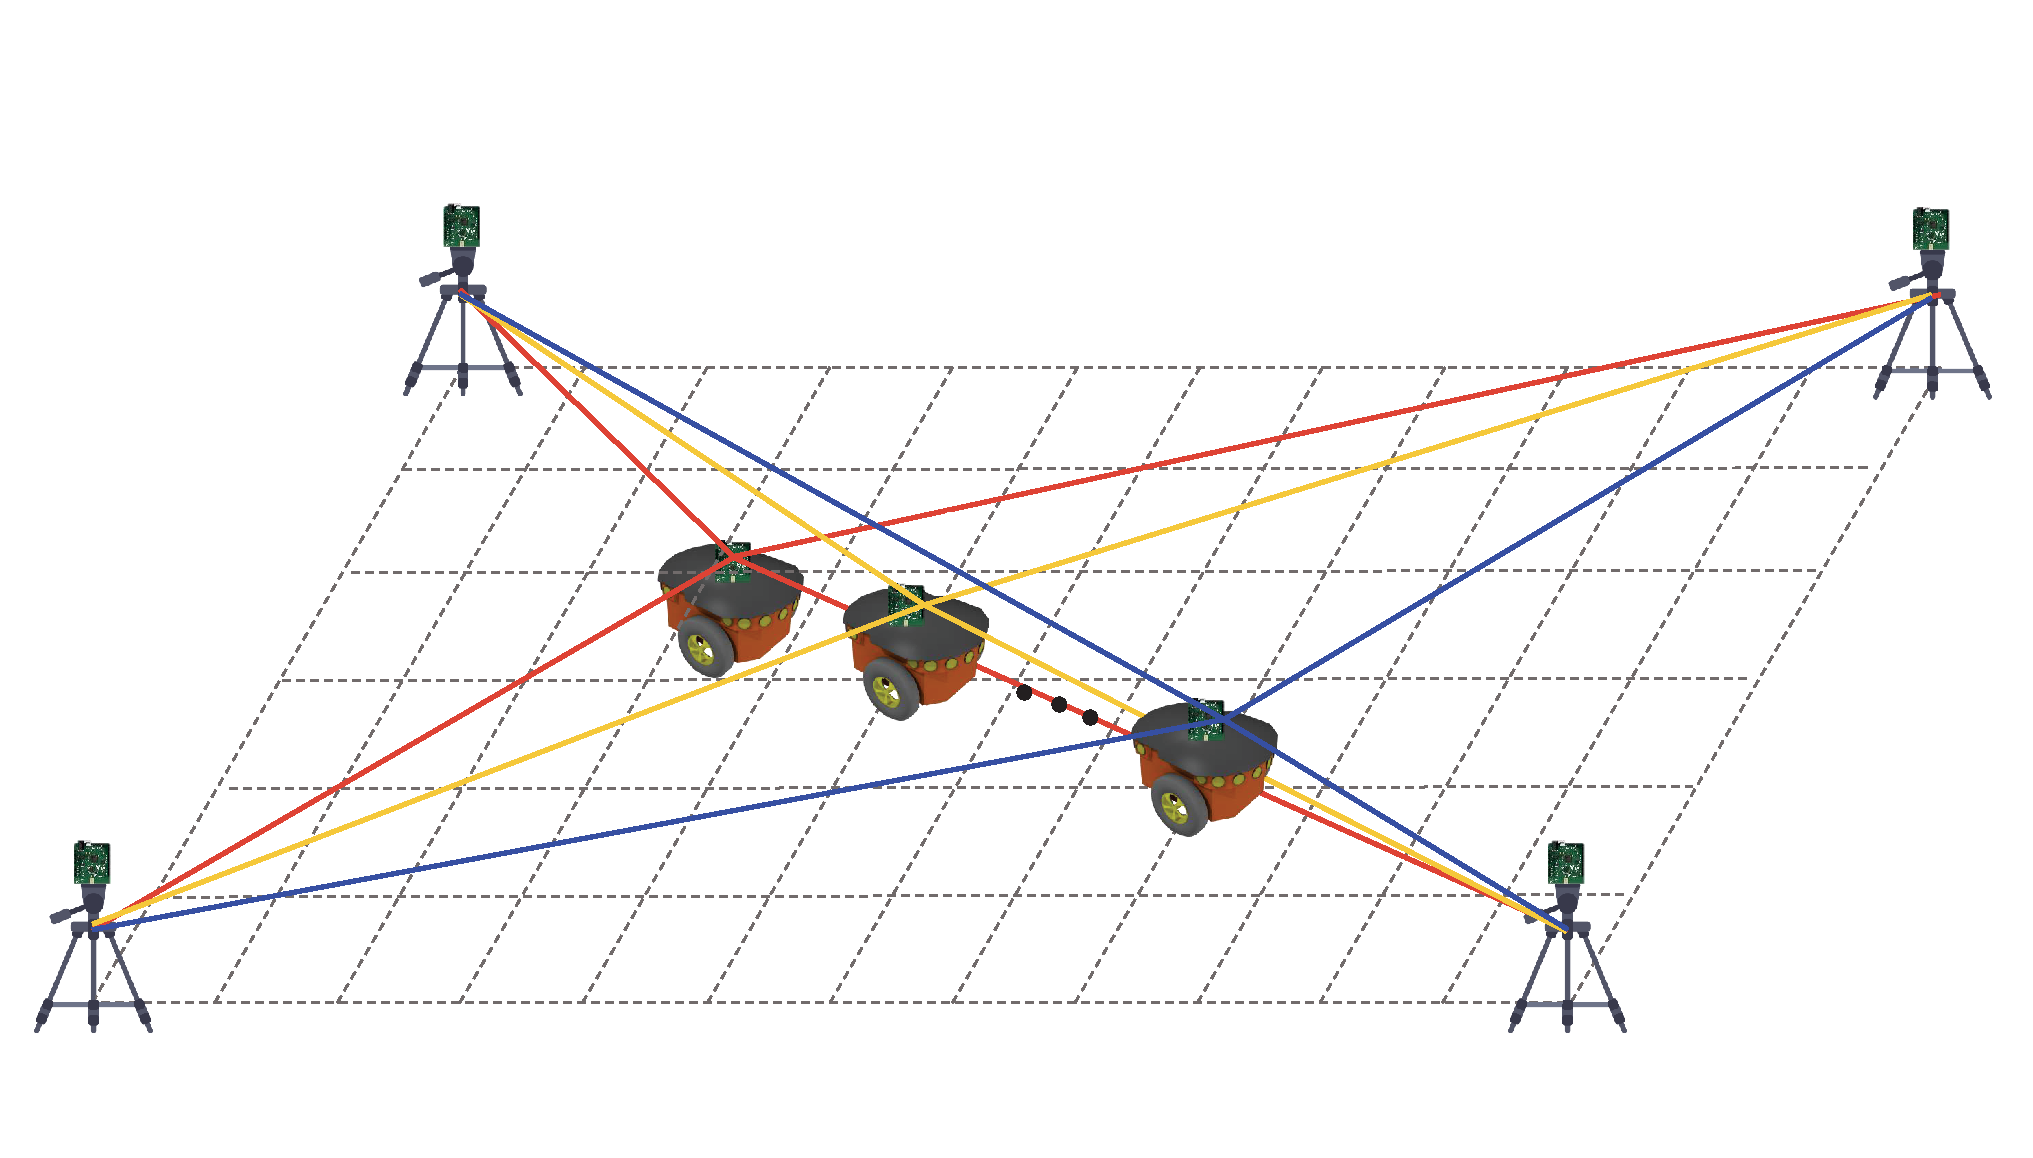
\includegraphics[trim={0 0 0 1cm}height=4.5cm]{IROS2018_image_1}
	\label{fig:overview}
	%	}
	
	\caption{Comparison between a conventional probabilistic-based range-only frameworks and our learning-based approach.}
	
\end{figure}

To alleviate these issues, many studies have been conducted based on probabilistic Bayesian inference frameworks and Monte-Carlo Bayesian filters, but in recent years, there have been attempts to solve these problems based on neural-network-based approaches\cite{rahman2009localization, abdelhadi2013efficient, kumar2016localization, lim2018effective}. With non-linear end-to-end mapping, the authors show feasibility. But most cases, the authors just utilized Multilayer Perceptron(MLP), which is beginning architecture of deep learning fields\cite{rahman2009localization, abdelhadi2013efficient, kumar2016localization}. In \cite{lim2018effective}, stacked bidirectional Long Short-Term Memory(Bi-LSTM) is implemented to cover the noise of range observation by utilizing the characteristics of it that takes temporal sequential value as input, yet they tested on the simulated environment. Besides, all of them are not checked whether their learning-based approaches are real-time or not. 

In this paper, we propose a robust stacked Bi-LSTM with residual attention, called RONet. To the best of our knowledge, it is a first approach to apply LSTM-based architecture to localize a mobile robot on the real-world in real-time using range-only measurement. Unlike conventional probabilistic-based algorithms, it does not need any preprocessing module, such as a calibration and outlier rejection.

Our contribution is threefold as follows:
\begin{itemize}
	%\setlength{\itemindent}{-.5in}
	\item We develop 3-stacked Bi-LSTM layers and attach residual attention layer for both improving performance and let the neural network be trained well so that our RONet shows the best performance when comparing the previous approaches.
	\item We also analyzed how the sequential length of the network affects performance and check robustness of our RONet with a minimal number of anchors.
	\item We operate RONet on Nvidia Jetson AGX Xavier and check the inference Hz is Real-time, about 32Hz. 
	
\end{itemize}

The rest of the paper is organized as follows: Section II overviews the related works. Section III describes our neural network in detail and defines the problem to be considered, and Section IV describes the experimental results. Finally, Section V summarizes our contributions and points to future work.

\section{Related Works}
\subsection{Conventional Range-Only Localization}

To localize a mobile robot using range measurements, there are two conventional approaches: Kalman Filter(KF)-based method and Particle Filter(PF)-based method. However, unlike other sensors, range measurements are hard to linear approximation because of MPF or Non-line of Sight issues(NLOS). So some authors insist that PF-based approaches could be better than KF-based approaches because PF can cope with complex non-linear model and also cover multimodal distributions\cite{gonzalez2009mobile, blanco2008pure,shetty2018particle}. 

Fig. 1. shows that general steps for conventional probabilistic approaches. First, each range measurements are need to be calibrated respectively. Then, after initialization, the algorithm check whether input value is outlier or not, and then eliminate this unexpectedly large noise. Next, they predict present states, including the mobile robot's pose and anchors' location and finally they correct their prediction using range observation.

 \begin{figure*}[h]
	\centering
	\includegraphics[width=0.95\linewidth]{image/network_figure}
	\caption{Our networks consists of three elements: Bi LSTM, the residual attention module(the blue cuboid), and fully-connected layer(FC layer). Features are fed in to Bi-LSTM and Bi-LSTM reduce feature in half, as 2048-1024-512. Finally, extracted features are fed in to FC layer to estimate position corresponding to each time step}
	\label{fig:our_network} 	
\end{figure*}

\subsection{LSTM-based Sequential Modeling}

As deep learning age has come\cite{lecun2015deep}, various kinds of deep neural architectures have been proposed for localization task \cite{kendall2016modelling, kendall2015posenet, gladh2016deep}. Especially, recurrent neural networks (RNNs), originated from the Natural Language Process(NLP) area\cite{elman1990finding}, have been shown to achieve better performance in case of dealing with time variant information. 

Besides, as Long Short-Term Memory (LSTM) architecture solves the \textit{long-term dependency}, which is the inherent issue to RNNs that become unable to learn the relationship of sequential information as the time-sequential gap grows\cite{hochreiter1997long}, LSTM are actively introduced to learn longer-term contextual understandings. Therefore, many authors exploit LSTM for sequential modeling after feature extraction by CNN\cite{clark2017vinet,patel2018contextualnet, wang2017deepvo}
 
\subsection{Deep Learning for Range Only Localization}

Specifically, LSTM are also utilized to model low-dimensional sensor data by itself. In \cite{wang2018deepml}, they exploit LSTM for indoor localization with magnetic and light sensors. And in \cite{chen2018ionet}, they estimate 2D odometries via stacked Bi-LSTM that takes only IMU sensor data as input. 

Our target, localization using range-only measurement, many authors employee neural networks-based approaches in Wireless Sensor Networks Fields(WSNs)\cite{rahman2009localization, abdelhadi2013efficient, kumar2016localization}, yet most networks are based on The MLP. Their approach only map a set of range observations on time $t$ to position so their approaches might have potential to unexpected sensor input. Other paper\cite{lim2018effective}, stacked bi-LSTM is implemented for localization a mobile robot takes sequential range measurements from anchors and the tag, but they only conducted simulation environment, which MPF or unexpected noises do not occur. Therefore, in this paper, we conduct experiments on a real-world to verify the workability to cover all noises of sensors with sequential range information and compare these approaches.

\subsection{Attention Layer}

A Attention layer is powerful module nowadays and mostly improves performance of neural network. Originally, neural networks treats information equally. But, using attention layer, neural networks can be ATTENDED what it should be examined closely, taking on a role as a feature selector\cite{wang2017residual}. On the first time, attention is utilized at the NLP areas for improving translation performance\cite{luong2015effective}. But nowadays, the attention layer is employed in many areas to improve the performance of the networks. 
 
 
 
\section{RONet}

In this chapter, we explain how our proposed residual attention-based stacked Bi-LSTM is implemented, as illustrated in Fig. \ref{fig:our_network}. 
In detail, we introduce the stacked Bi-LSTM and residual attention module that we choose for localizing the tag node and then compare to those of other previous works. Finally, we describe how to set the loss function of our neural network. 

\subsection{Long Short-Term Memory}

Unlike RNN that consist only of hidden state, in LSTM, cell state is added to the network. The cell state consists of 3 gates to preserve the previous information and control the cell state: the forget gate, input gate, and output gate and equations of those are as follows:


\begin{align}
f_{t} & =\sigma _{s}\big(W_{xf}\cdot x_{t}+W_{hf}\cdot h_{t-1}+b_{f}\big)\label{eq:forget}\\
i_{t} & =\sigma _{s}\big(W_{xi}\cdot x_{t}+W_{hi}\cdot h_{t-1}+b_{i}\big)\label{eq:input}\\
\tilde{c}_{t} & = \tanh\big(W_{xc}\cdot x_{t}+W_{hc}\cdot h_{t-1}+b_{c}\big)\label{eq:new_cell}\\
c_{t} & =f_{t}\odot c_{t-1}+i_{t}\odot\tilde{c}_{t}\label{eq:update}\\
o_{t} & =\sigma _{s}\big(W_{xo}\cdot x_{t}+W_{ho}\cdot h_{t-1}+b_{o}\big)\label{eq:output}\\
h_{t} & =o_{t}\odot \tanh\big(c_{t}\big)\label{eq:hidden}
\end{align}

where $\sigma _{s}$ is a kind of activation function, called \textit{sigmoid},  $f_{t}$, $i_{t}$, and $o_{t}$ respectively indicates the forget gate, input gate, and output gates, and $c_{t}$ denotes cell states. And $\odot$ denotes element-wise multiplication, called \textit{Hadamard product}. The entire gates are activated by sigmoid function and cell states are activated by $\tanh$ function.

The Forget gate layer, $f_{t}$, decides how much information to forget based on the previous hidden state, $h_{t-1}$, and present input, $x_{t}$. Next, the input gate, $i_{t}$, decides how much information to embrace when updating the cell state. After that, $c_{t}$ is updated by the cell state layer based on $f_{t}$, $i_{t}$, and candidate cell state, $\tilde{c}_{t}$ \eqref{eq:update}. In addition, output gate layer, $o_{t}$, sereves as a filter, which means $o_{t}$ determine what values are going to output \eqref{eq:output} in such a way as that $h_{t}$, is updated based on $o_{t}$ updated cell state, $c_{t}$ \eqref{eq:hidden}. 

\subsection{Stacked Bidirectional LSTM}

\begin{figure}[h!]
	\centering
	\includegraphics[width=.9\linewidth]{image/bidirectional_LSTM_revised}
	\caption{Architecture of the Bidirectional LSTM(Bi-LSTM). bidirectional LSTM consist of 2 LSTMs:  one forward LSTM layer}
	
	%$\overrightarrow{LSTM}$, and one backward LSTM layer, $\overleftarrow{LSTM}$}
	\label{fig:bidirectional_revised}	
\end{figure}

Like the fact that the deeper the architecture of neural networks, the better their performance\cite{simonyan2014very, he2016deep}, many authors have analyzed variations of LSTM architecture and find out that stacking multiple layers of the LSTM improve the performance for many tasks\cite{graves2013hybrid, graves2013speech,ullah2018action}. Besides, Bidirectional RNNs are introduced\cite{schuster1997bidirectional} to extract well-described context. It has one forward LSTM, $\overrightarrow{LSTM}$, and one backward LSTM, $\overleftarrow{LSTM}$, running in reverse time so that the network exploits not only the previous forward context to up update $h_{t}$ and $c_{t}$ but also future backward context as well, as FIGURE. \ref{fig:bidirectional_revised} shown. 

For these reasons, we decide to implement the stacked Bi-LSTM architecture to model the system. By virtue of the increased non-linearity caused by a number of stacked layers, the network could model more complex localization taking UWB-ranging observations as input, which includes unexpected noise and MPF problems. Furthermore, we judge that Bi-LSTM would be more helpful to produce more appropriate context considering both past and future at the same time

Therefore, we construct our networks by stacking three LSTM to increase the non-linearity. Note that stacking over than three LSTM doesn't show the improvement of performance. We deem that this problem could come from the sigmoid function and $tanh$ function that compose the part of LSTM. These activation functions cause the \textit{vanishing gradient problem}\cite{pascanu2013difficulty}, which the networks fail to training due to the fact that the gradient is getting closer to zero during the backpropagation. Consequently, we put the Rectified Linear Unit(ReLu) function between LSTMs to avoid the vanishing gradient problem\cite{nair2010rectified}, instead of stacking more LSTM to increases non-linearity. In addition, experiments shows that reducing the hidden size of the next LSTM layer when the features are fed into the LSTM layer slightly increases performance, but reducing dramatically rather cause under-fitting. In conclusion, we decide to set the size of the layers as 1024-512-128. Note that we adopt Bi-LSTM, actual feature size is 2048-1024-256. The end part of the LSTMs, fully connected layers are attached to predict the mobile robot's position based on the sequential features processed by the LSTMs.  

\subsection{Residual Attention layer}

To precisely estimate the position of the tag node, it is important for the network to distinguish which is a more meaningful context on time step \textit{T} to help contextual understanding of our networks. The equation of original attention mechanism is as follows:  

\begin{equation}
H(x)=M(x)\odot x
\end{equation} 

where $x$ denotes the output of the previous neural network layer, $H(x)$ denotes the output of the attention layer to be passed to the next neural network layer and $M(x)$ denotes the attention mask. By element-wise multiplying $x$ by $M(x)$, attention layer makes the network weight more crucial information. 

Despite of the improvement of the performance, the attention layer has potential risks that it may dilutes the features because attention mask ranges over 0 to 1. So we adopt residual attention layer to alleviate this problem as follows\cite{wang2017residual}:

\begin{equation}
H(x)=\left(1+M(x)\right)\odot x
\end{equation} 

As blue cuboid shape in the FIGURE \ref{fig:our_network} shown, this idea is originated from the Residual Net(ResNet)\cite{he2016deep} that has skip connection in such a way as to mitigate aforementioned dilution problem and help the network to be trained well. Likewise the ResNet, residual attention also has other branch to calculate how much to attend and the branch is joined with original feature vector $x$. Each hidden state has each residual attention layer so that these attention modules can determine which time stamp has more fruitful meaning and deliver the output to next bidirectional LSTM.

\subsection{Training loss}

In this section, we describe the method for training our network. Generally, let $n$ be the number of anchor nodes, data set, $L_{t}$, measured by each anchor node and tag node and ground truth of 2D position, $Y_t$, are represented on the time step $t$ as follows:

\begin{equation}
L_{t} = (l_{1}, l_{2}, ..., l_{n})_{t}
\end{equation}
\begin{equation}
Y_t = (x_t, y_t)
\end{equation}

where $l_{i}$ denotes the the distance between $i^{th}$ anchor node and the tag node. Note that our neural network does not only take a set at the time $t$ but takes sets based on the sequential length of input to our network, $T$ as follows:

\begin{equation}
%$L = \left\{(X_t, Y_t)\right \}$ 
\mathbb{L}_t = \left\{L_{t-T+1}, L_{t-T+2}, ..., L_t\right\} 
\end{equation}
\begin{equation}
\mathbb{Y}_t = \left\{Y_{t-T+1}, Y_{t-T+2}, ..., Y_t\right\}
\end{equation}

Conseqeuntly, neural network could be optimized to be able to localize the mobile node by being trained using the train data set $\mathbb{D}$ as follows:  

\begin{equation}
%$L = \left\{(X_t, Y_t)\right \}$ 
\mathbb{D} = \left\{(\mathbb{L}_{T-1}, \mathbb{Y}_{T-1}),...,(\mathbb{L}_t, \mathbb{Y}_t),...\right\} 
\end{equation}

Therefore, Let $\Theta$ be the parameters of our network model and our final goal is to find optimal parameters $\Theta^{*}$ for precise localization by minimizing $L_2$ loss term. The $L_2$ loss term indicates mean square error(MSE) of Euclidean distance between the normalized ground truth position $\mathfrak{N}(Y_k)$ and estimated position $\hat{Y_k}$ as follows:

\begin{equation}
\Theta^{*} = \underset{\Theta}{\mathrm{argmin}} \frac{1}{N}\frac{1}{T} \sum_{k=T-1}^N\sum_{m=k-T+1}^k \parallel \mathfrak{N}(Y_m) - \hat{Y_m} \parallel^{2}
\end{equation}  

\begin{figure*}[h]
	\centering
	\begin{subfigure}[b]{0.32\textwidth}
		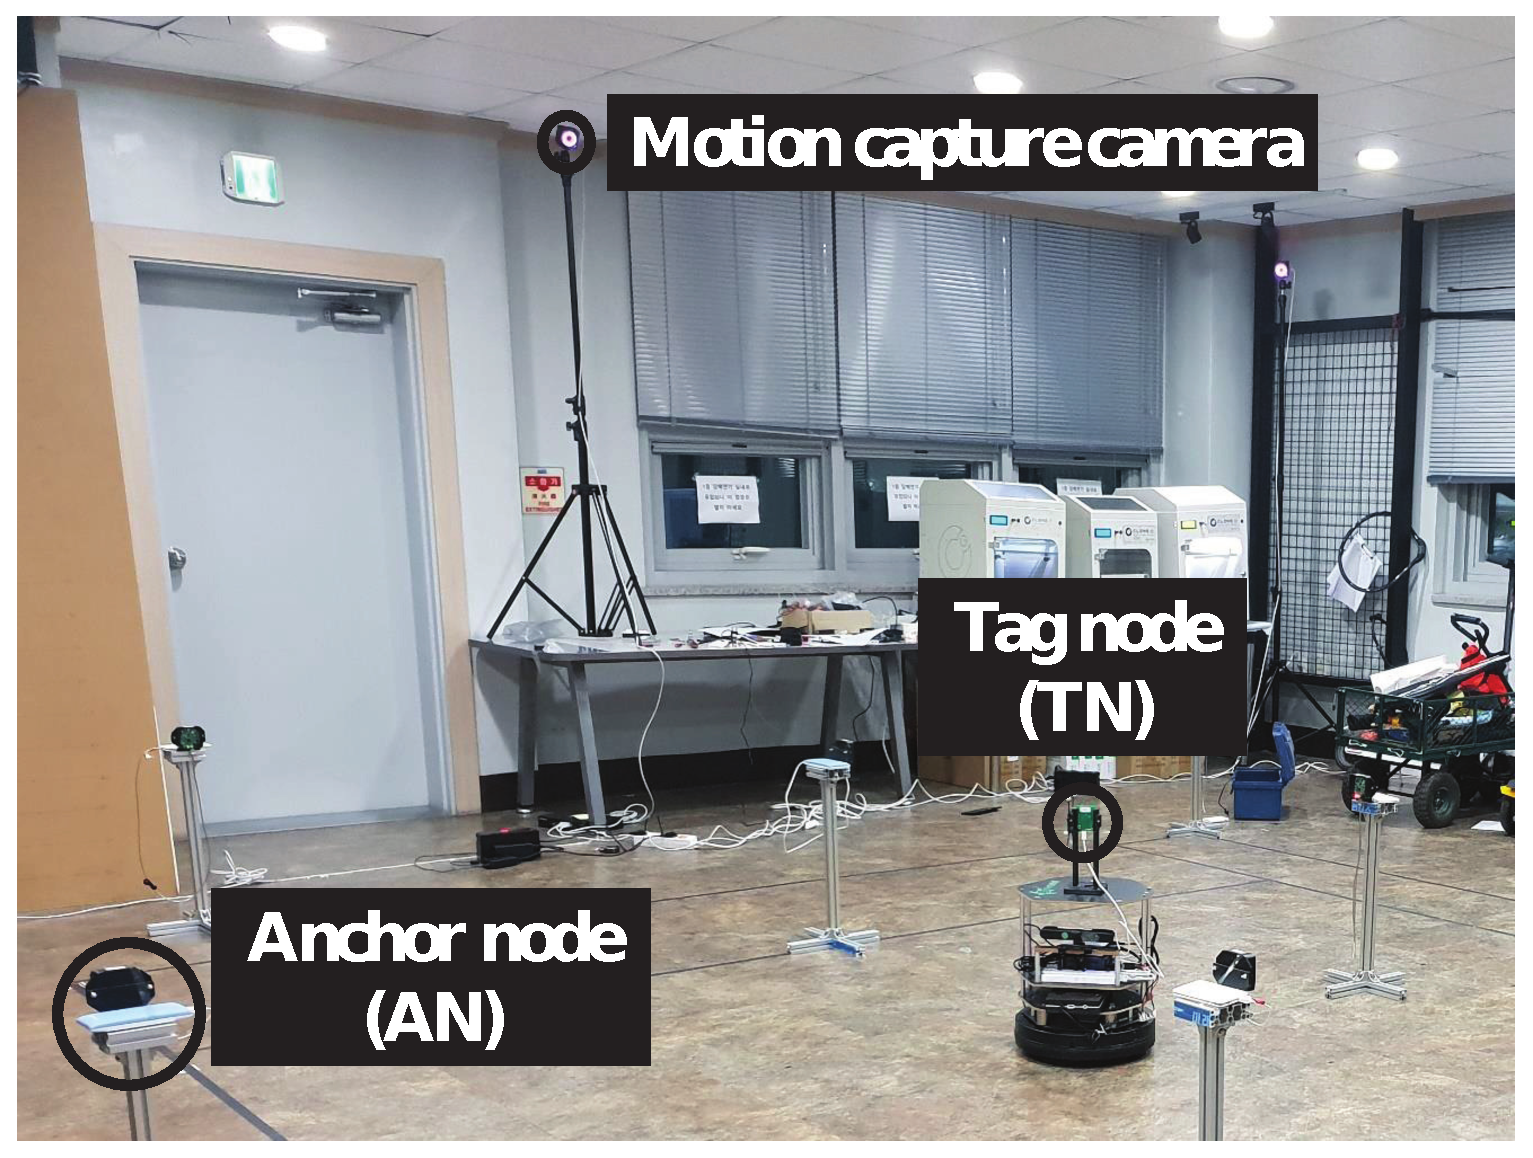
\includegraphics[width=\textwidth]{image/system_whole_picture}
		\caption{}
		\label{fig:whole_system}
	\end{subfigure}
	%add desired spacing between images, e. g. ~, \quad, \qquad, \hfill etc. 
	%(or a blank line to force the subfigure onto a new line)
	\begin{subfigure}[b]{0.32\textwidth}
		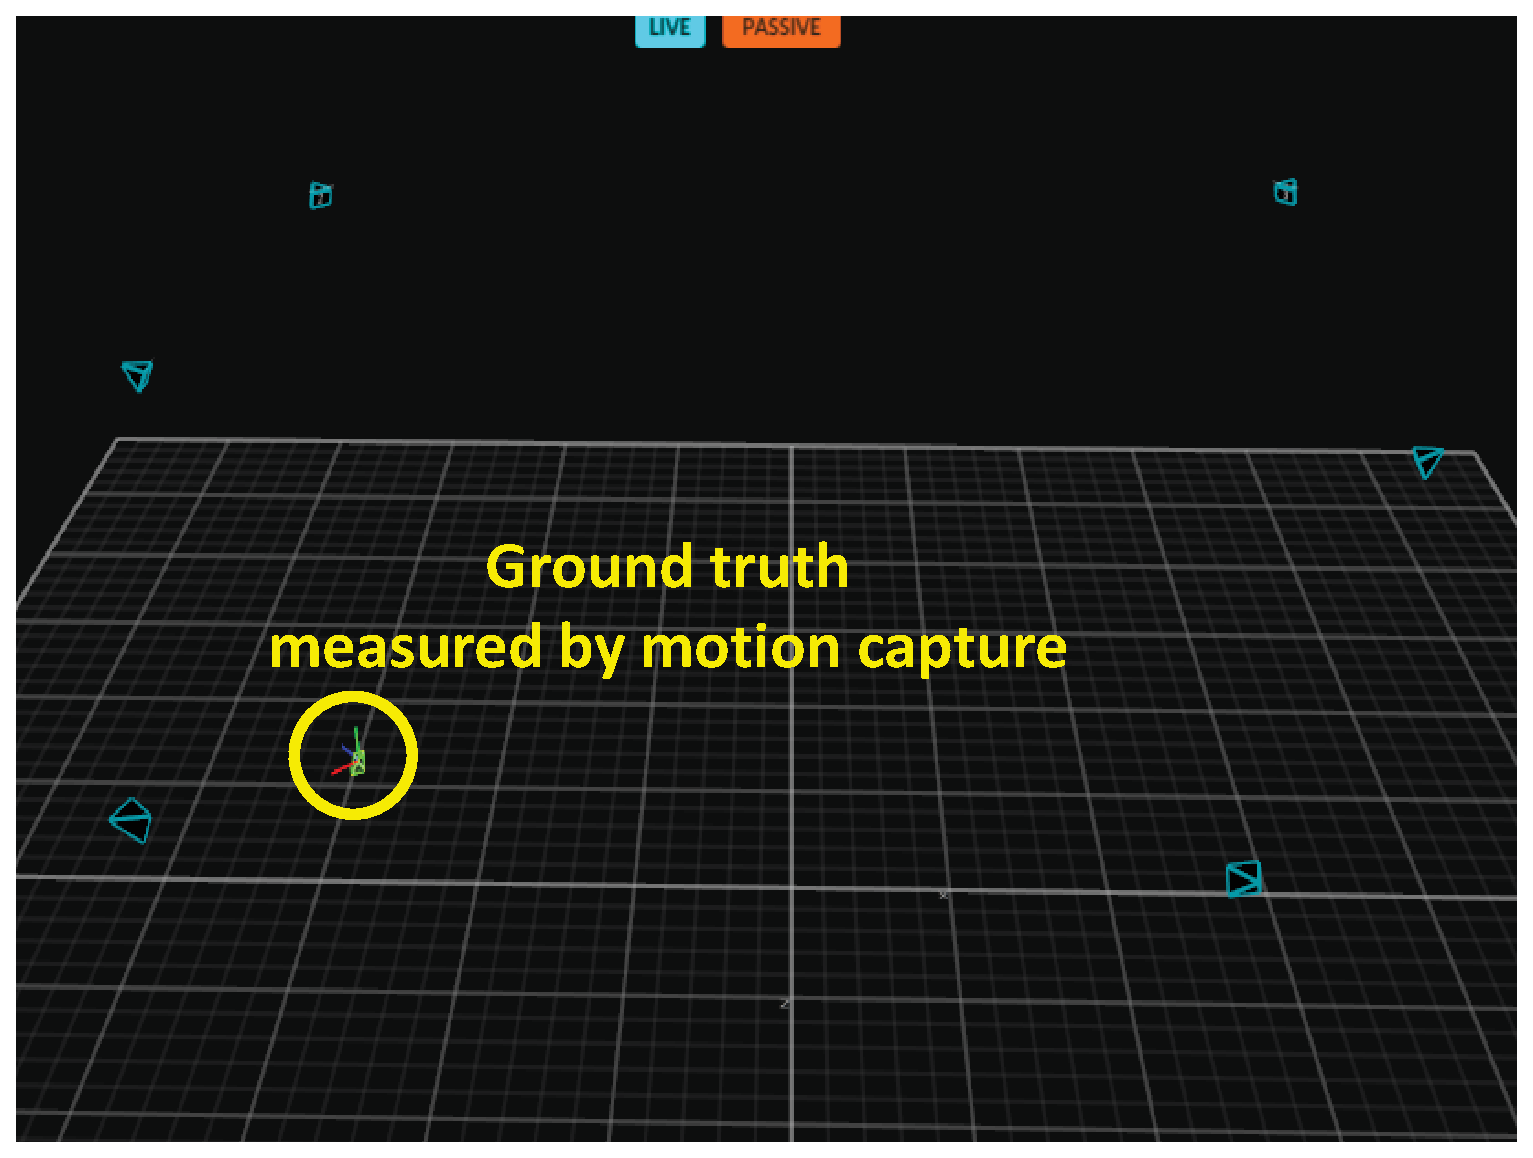
\includegraphics[width=\textwidth]{image/system_mocap}
		\caption{}
		\label{fig:Optitrack_figure}
	\end{subfigure}
	%add desired spacing between images, e. g. ~, \quad, \qquad, \hfill etc. 
	%(or a blank line to force the subfigure onto a new line)
	\begin{subfigure}[b]{0.32\textwidth}
		\includegraphics[width=\textwidth]{image/system_exact_position}
		\caption{}
		\label{fig:Exact_position}
	\end{subfigure}
	\caption{(a): entire experimental environments, (b): tracked pose from Optitrack motion capture, and (c): exact position of anchor nodes. }\label{fig:animals22}
\end{figure*}

\section{Experimental Results}
\subsection{Experimental environment}

Our experimental system consists of a UWB sensor tag node attached on the mobile robot platform  and eight anchor nodes that take roles of a UWB transceiver, 6 Optitrack Prime 13 motion capture cameras, a Nvidia Jetson AGX Xavier, which is a SFF(small-form-factor) computer that has a GPU. Fig. \ref{fig:whole_system} shows our experimental environment briefly and how to the anchor nodes and the tag node are attached. And we use the mobile platform, called iClebo Kobuki from Yujinrobot.

The tag node receives the signal and measures the range between two devices based on time of flight(TOF) and Received Signal Strength Indication(RSSI). Each UWB transceiver, DW1000 UWB-chip made by Decawave, supports 6 RF bands from 3.5 GHz to 6.5 GHz. It measures in cm-level accuracy.

 %Deep learning framework used for our network is tensorflow-gpu 1.7.0 on python 3.5.2
 
\subsection{Acquisition of the Train/Test data}
UWB sensor anchors are installed randomly in the region where motion capture camaras are acceptable, as Fig. \ref{fig:Exact_position} shown. These anchor nodes transmit the UWB signal to tag node that is attached to the mobile robot and the Optitrack motion capture cameras also transmit the ground truth data to the SSF computer by utilizing Robot Operating System(ROS).

Note that these two data are transmitted by different frequency: range measurements are gathered with a frequency of almost 27Hz, yet the ground truth data are 120Hz. So we synchronize these two data based on the range measurements' Hz. More specifically, we set an independent thread so that this thread select the ground truth data of the nearest time based on the UWB-range measurements, concatenates and saves these data at the same time.

And the mobile robot moves in this space by manually. All the trajectories are different. After collecting whole datasets, we separate the entire dataset to three types: one are the training datasets, another are for the validation datasets, and the other is for test dataset. On the test dataset, only range measurements are taken as input to the network.

\subsection{Training the Network}

To optimize our network, the Adam optimizer is exploited to train the
network during 1200 epochs with 0.001 learning rate, 0.9
decay rate, and 5 decay step. And we found that network is influenced by batch size: when the batch size is too large, the performance of filtering unexpected noise of sensors is reduced by its over-generalizing. On the other hand, when the batch size is too small, the network tend to be overfitted to train data's specific noise pattern. Therefore, we set moderated-sized batch size as 6355.
 

\subsection{Localization Results}

\subsubsection{The Performance according to the sequence length}

\begin{figure}[h!]
	\centering
	\includegraphics[width=0.9\linewidth]{image/RMSE_error}
	\caption{RMSE graph of RMSE w.r.t. the sequence length by changing the number of anchors}
	\label{fig:seq_length_on_different_anchors} 	
\end{figure}

We also considered the sequence length as a kind of hyper-parameters. We checked the effectiveness of optimal size of the sequence length in three cases by changing the number of range input data. As fig. \ref{fig:seq_length_on_different_anchors} shown, there's no surprising that performance is improved when the more number of sensors value is taken as input, but as the sequence becomes longer, the network improves overall performance through more fruitful temporal information.

As a result, we found that there is a trade-off between robustness and generalization performance according to the sequence length. The network with longer sequence length tends to have less error variance and more an ability to generalize the situation since they could utilize more extended temporal information. By doing so, the neural network gets the ability to suppress the disturbance caused by noises. 

However, note that the performance when the network is implemented to 12 sequence length is rather a little bit inaccurate than that of 8 sequence length. This is because of accumulations of different patterns of sensor noises as the number of anchors increases. In other words, the tendency of domain values may become different due to accumulations of different patterns of sensor noises even though a part of the test data path is a similar to the path in the train data. That's the reason why as sequence length become longer, range observations included in test data are hard to be mapped correctly based on the training.

For these reasons, we set optimal sequence length as 8 with considering these two aspects, abilities that both cover uncertainty with more temporal information and estimate position precisely.

%Similarily, as sequence length become shorter, it is less difficult for the neural architecture to understand the chracteristics of the sequential data by virtue of the less accumulation of different patterns of system noises. Note that in most cases, the network constructed by the shorter sequential length tend to estimate the position more precisely than those with longer sequential lengths. However, 생t becomes a double-edged sword because temporal information is also reduced accordingly in such a way as to week to the noises, having larger error variance.



%sequence length가 길어질수록 netowrk가 그 sequential data를 일반화 시키는 게 어렵다
%In other workds, sequence length만큼 끊어서 input으로 받기 때문에 sequential한 경향성에 대해 적절한 output을 내게 학습을 하는데, sequence가 길어지게 되면 길어지는 만큼 그 상황이 특수해져서 비슷한 특성을 지닌 input이 줄기 때문이다????
%길이가 길어짐에 따라 noise에 대한 방해를 더 길어진 temporal information을 활용해서 억누를 수 있다.
%On the other hand, 짧아질수록 좋지만 경향성을 학습?

\subsubsection{The Performance comparison of Other Algorithms}

We also compared our network with recently presented learning-based approaches, MLP\cite{kumar2016localization} and Bi-LSTM\cite{lim2018effective}, and the conventional PF-based approach. We implemented PF-based localization by referring \cite{gonzalez2009mobile}. We tested on various number of anchors in such a way as to check if the algorithms work well on the environment that the number of range sensors is small so the algorithms are more affected by the sensor noise.

\begin{figure}[h]
	\centering
	\includegraphics[width=0.9\linewidth]{image/boxcompare}
	\caption{Box plot results with respect to the number of anchors.}
	\label{fig:box_plot} 	
\end{figure}

\begin{table}[h]
	\centering
	\caption{Root Mean Square Error of each algorithm w.r.t. the number of anchors}
	\begin{tabular}{ccccc}
		\hline
		\multicolumn{5}{c}{The results of RMSE {[}cm{]}}   \\ \hline
		\# of anchors & Particle Filter\cite{gonzalez2009mobile} & MLP\cite{kumar2016localization} & Bi-LSTM\cite{lim2018effective} & Ours \\ \cline{2-5} 
		3             & 8.722 & 5.485 & 5.051 & \textbf{4.466} \\
		5             & 8.286 & 4.546 & 4.418 & \textbf{3.210} \\
		8             & 7.650 & 4.235 & 4.290 & \textbf{3.090} \\ \hline
	\end{tabular}
	\label{table:rmse}
\end{table}



\begin{figure*}[h]
	\centering
	\begin{subfigure}[b]{0.32\textwidth}
		\includegraphics[width=\textwidth]{image/trajectory_3}
		\caption{}
		\label{fig:anchor_3}
	\end{subfigure}
	%add desired spacing between images, e. g. ~, \quad, \qquad, \hfill etc. 
	%(or a blank line to force the subfigure onto a new line)
	\begin{subfigure}[b]{0.32\textwidth}
		\includegraphics[width=\textwidth]{image/trajectory_5}
		\caption{}
		\label{fig:anchor_5}
	\end{subfigure}
	%add desired spacing between images, e. g. ~, \quad, \qquad, \hfill etc. 
	%(or a blank line to force the subfigure onto a new line)
	\begin{subfigure}[b]{0.32\textwidth}
		\includegraphics[width=\textwidth]{image/trajectory_8}
		\caption{}
		\label{fig:anchor_8}
	\end{subfigure}
	\caption{Trajectories results with respect to the various number of anchors: (a): a trajectory with 3 anchors, (b): a trajectory with 5 anchors, (c): a trajectory with 8 anchors. For clarity, we just drawed PF-based results(organge) and our RONet results(blue).}\label{fig:trajectories_358}
\end{figure*}

As Fig. \ref{fig:box_plot} and Table. \ref{table:rmse} are shown, our RONet show the best performance among both the conventional algorithm and previous deep learning-based approaches in all cases. It shows the least Root Mean Square Error(RMSE), which RONet's RMSE is 4.466cm, 3.210cm, 3.090cm in order of 3 anchors, 5 anchors, and 8 anchors are implemented respectively. Furthermore, it also shows that our network estimate position with smaller outliers than other algorithms. 

\section{Conclusion}

In this paper, we propose a robust 3-stacked BI-LSTM with residual attention, called RONet. We tested our approaches in real-world and it shows that it could estimate a position of the mobile robot in real-time, almost 32Hz, using range-only measurement. Unlike conventional probabilistic-based algorithms, it does not need any preprocessing module, such as a calibration and outlier rejection because it maps between range observation and position by end-to-end.

In addition, We also analyzed the sequence length as a kind of hyper-parameters. We conclude that 8 sequence length is optimal among 2,3,5,8, and 12 sequence lengths in the way that building the network with 8 sequence length compromise both abilities that cover uncertainty with more temporal information and estimate position precisely.

Finally, we compare other conventional probabilistic approach and previously presented deep learning-based algorithms with our RONet and RONet exhibits the most precise estimates of robot positions. We set three cases, reducing the number of anchors and check that our RONet is not only robust but also shows the least RMSE, 4.466cm, 3.210cm, 3.090cm in order of 3 anchors, 5 anchors, and 8 anchors are implemented respectively. 

As a future work, because we conducted on just localization, this approach may not be operated when locations of sensors are arbitrary placed. Therefore, the proposed method, e.g., loss term or architecture of the neural network needs to be revised for precise estimates even though locations of anchors are changed. 

\bibliographystyle{IEEEtran}
% argument is your BibTeX string definitions and bibliography database(s)
\bibliography{./IEEEabrv,./IROS_RObib}


\end{document}
